\documentclass[conference]{IEEEtran}

\usepackage[T1]{fontenc}
\usepackage{newtxtext,newtxmath}
\usepackage{graphicx}
\usepackage{booktabs}
\usepackage{amsmath}
\usepackage{url}
\usepackage{balance}
\usepackage[hidelinks]{hyperref}

\usepackage{tikz}
\usetikzlibrary{arrows.meta,positioning,fit,backgrounds,calc}

\newcommand{\rupee}{INR\,}

% Figure palette: the validated categorical slots, shared by the TikZ
% flowcharts and by scripts/make_short_paper_figures.py, so a colour means
% the same thing in a diagram as it does in a chart.
\definecolor{vblue}{HTML}{2A78D6}
\definecolor{vorange}{HTML}{EB6834}
\definecolor{vaqua}{HTML}{1BAF7A}
\definecolor{vyellow}{HTML}{EDA100}
\definecolor{vviolet}{HTML}{4A3AA7}
\definecolor{vink}{HTML}{0B0B0B}
\definecolor{vmuted}{HTML}{52514E}

\tikzset{
  vbox/.style={
    rounded corners=1.6pt, draw=#1, line width=0.5pt, fill=#1!10,
    text=vink, align=center, inner sep=2.2pt, font=\scriptsize},
  vband/.style={
    rounded corners=3pt, draw=#1!30, line width=0.5pt, fill=#1!4,
    inner sep=4pt},
  vhead/.style={text=#1, font=\scriptsize\bfseries, align=center},
  vflow/.style={-{Stealth[length=4.4pt,width=3.6pt]}, draw=vmuted,
    line width=0.75pt},
  vnote/.style={text=vmuted, font=\tiny, align=center},
}

\IEEEoverridecommandlockouts

\begin{document}

\title{Varuna FloodTwin: Urban Flood Digital Twins from\\
Free Satellite Data, and How to Score Them}

\author{
\IEEEauthorblockN{Ansh Vivek}
\IEEEauthorblockA{\textit{B.Tech, VLSI Design and Technology}\\
\textit{Vellore Institute of Technology}\\
Vellore, India\\
ansh.vivek2024@vitstudent.ac.in}
\and
\IEEEauthorblockN{Sumathi G}
\IEEEauthorblockA{\textit{School of Electronics Engineering}\\
\textit{Vellore Institute of Technology}\\
Vellore, India\\
sumathi.g@vit.ac.in}
}

\maketitle

\begin{abstract}
Indian cities flood every monsoon, and most of them have no calibrated flood model to plan with. We
present Varuna FloodTwin, an open pipeline that builds a flood model of any area from free satellite
data. The model runs fast enough to answer questions inside a web page, and it is deployed for 16
city areas in India on free computing services. While testing it, we found that the standard
accuracy score for this task is hard to interpret on its own. On 150 Sentinel-1 radar scenes across
15 areas, a baseline with no physics and no rainfall, which simply predicts the cells that were wet
in most other storms, scores a Critical Success Index (CSI) of 0.29 to 0.67. This is higher than
every published physics-model score we could find, including our own, and in all 15 areas it is
higher than the agreement between two radar passes over the same city. A neural network trained on
the same terrain maps scores 0.288 and ties this baseline to three decimal places. Its value is that
it can also run on cities with no radar history. On regions held out from training it scores 0.147,
and a threshold correction that never sees a test label raises this to 0.175. Adding one coastal
city to training improves the score on held-out coastal Mumbai by 84\,\%. A larger model, a finer
grid and free rainfall data did not help. Planning still works under this uncertainty, because we
value each intervention by running the storm again over the changed ground. A dense storm drain
network routed along real streets removes 80.9\,\% of simulated street flooding in Patna, at a lower
cost per cubic metre than sparse canals. A recharge planner sends 6.3 to 16.5\,\% of storm runoff
into the aquifer in six depleted Karnataka towns, against 0.7 to 3.3\,\% on the Patna flood plain.
\end{abstract}

\begin{IEEEkeywords}
Urban flooding, digital twin, Sentinel-1, flood validation, managed aquifer recharge, open data.
\end{IEEEkeywords}

\section{Introduction}
\IEEEPARstart{P}{luvial} flooding is flooding caused by rain falling on a city, as opposed to a
river spilling over its banks. It is one of the most common climate impacts in South Asian cities.
Most Indian municipalities plan for it with a drainage map that is older than the city around it.
They have no calibrated hydraulic model and no budget to buy one. A flood tool that could help in
this setting has to be built from free global data, because nobody is going to survey the city for
it. It should be cheap enough to use interactively, so that a planner can try an idea and see the
result straight away. It should also be clear about what it cannot predict, since a confident wrong
answer about which street floods can be worse than no answer.

\begin{figure}[!t]
\centering
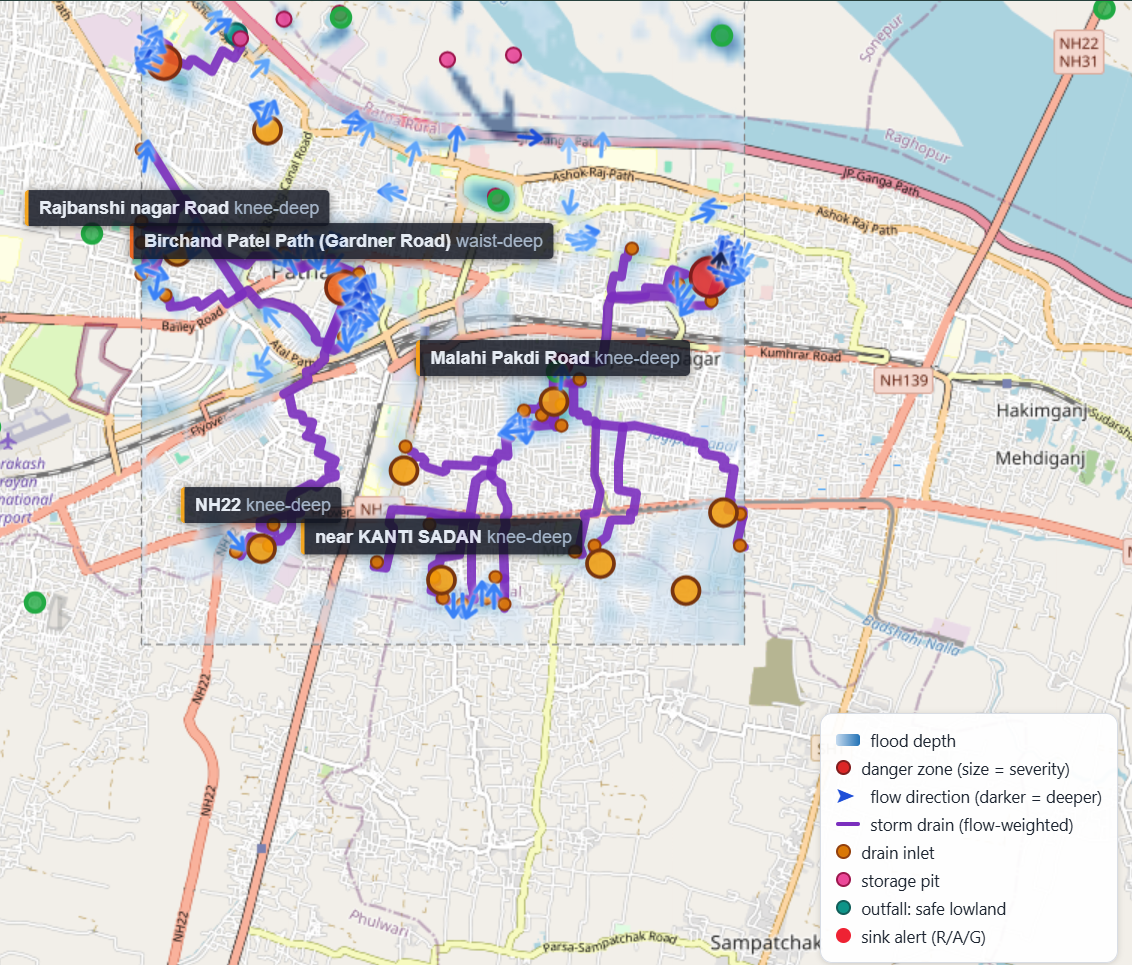
\includegraphics[width=0.90\linewidth]{figures/live_patna_city.png}
\caption{The live system for Patna under a 100\,mm design storm. Blue shows predicted depth and the
arrows show the direction of flow. Purple lines are the drain network that the planner designed on
the real street graph. Labels name real streets and describe their depth in words.}
\label{fig:teaser}
\end{figure}

Varuna FloodTwin is our attempt at such a tool. It builds a digital twin of a city area, meaning a
simulation of that particular place which can be run again under any storm or after any change to
the ground. Fig.~\ref{fig:teaser} shows what a planner sees, and Fig.~\ref{fig:pipeline} shows the
whole pipeline. Free satellite data becomes a flood model in 15 to 25 minutes on a free GPU. The
model is scored against Sentinel-1 radar images of real storms, and it is then used to test drains,
storage tanks and recharge basins.

The most important result in this paper came from the scoring step. When we computed simple
baselines on the same radar scenes as our model, a baseline with no model at all scored far higher
than our physics model, and higher than any physics-model score we could find in the literature.
Section~\ref{sec:worth} describes this in detail. It means that a flood score reported without such
baselines says very little, and it changes how the rest of our results should be read.
Section~\ref{sec:twin} compares the physics model with a learned model. Section~\ref{sec:transfer}
tests the learned model on places it has not seen, and Section~\ref{sec:levers} reports three
changes that did not help. Section~\ref{sec:planning} describes planning, and
Section~\ref{sec:limits} lists the limitations of this work.

\begin{figure*}[!t]
\centering
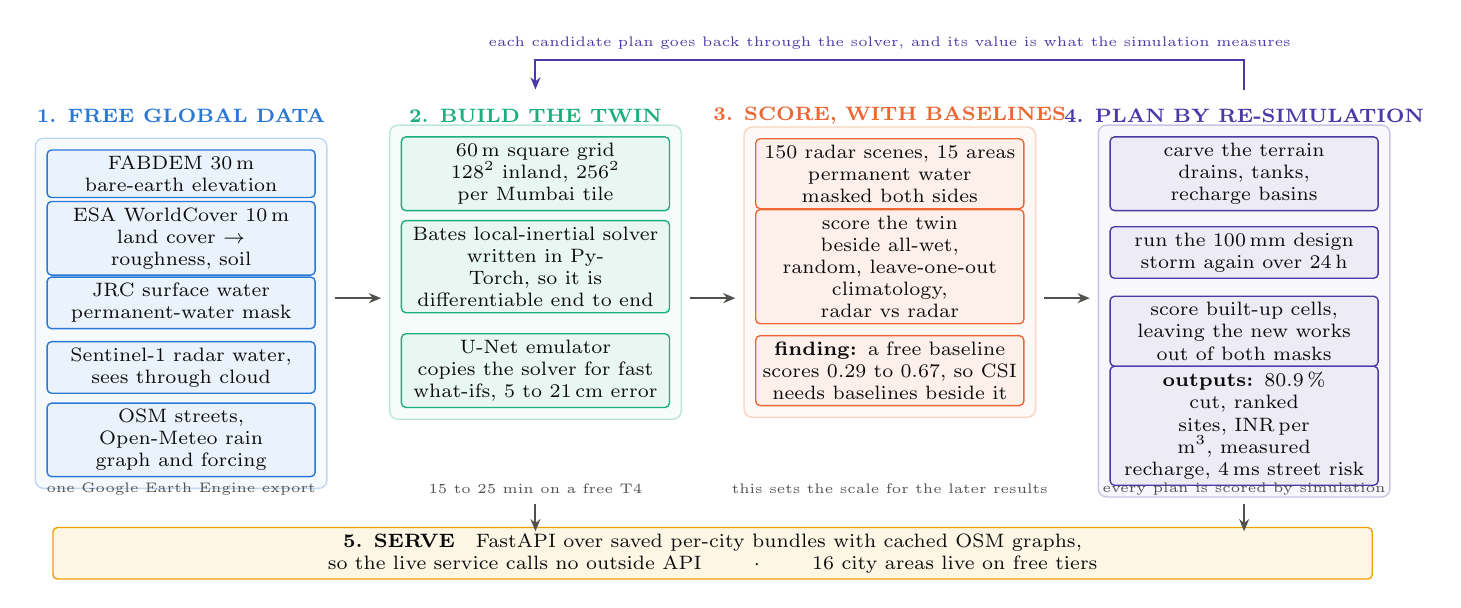
\begin{tikzpicture}[x=1cm,y=1cm]

% stage 1: free global data
\node[vhead=vblue] at (2.0,0.42) {1. FREE GLOBAL DATA};
\node[vbox=vblue,text width=3.25cm] (a1) at (2.0,-0.32)
  {FABDEM 30\,m\\bare-earth elevation};
\node[vbox=vblue,text width=3.25cm] (a2) at (2.0,-1.14)
  {ESA WorldCover 10\,m\\land cover $\rightarrow$ roughness, soil};
\node[vbox=vblue,text width=3.25cm] (a3) at (2.0,-1.96)
  {JRC surface water\\permanent-water mask};
\node[vbox=vblue,text width=3.25cm] (a4) at (2.0,-2.78)
  {Sentinel-1 radar water,\\sees through cloud};
\node[vbox=vblue,text width=3.25cm] (a5) at (2.0,-3.70)
  {OSM streets, Open-Meteo rain\\graph and forcing};
\node[vnote] at (2.0,-4.32) {one Google Earth Engine export};

% stage 2: build
\node[vhead=vaqua] at (6.5,0.42) {2. BUILD THE TWIN};
\node[vbox=vaqua,text width=3.25cm] (b1) at (6.5,-0.32)
  {60\,m square grid\\$128^2$ inland, $256^2$ per Mumbai tile};
\node[vbox=vaqua,text width=3.25cm] (b2) at (6.5,-1.50)
  {Bates local-inertial solver\\written in PyTorch, so it is\\differentiable end to end};
\node[vbox=vaqua,text width=3.25cm] (b3) at (6.5,-2.82)
  {U-Net emulator\\copies the solver for fast\\what-ifs, 5 to 21\,cm error};
\node[vnote] at (6.5,-4.32) {15 to 25 min on a free T4};

% stage 3: score
\node[vhead=vorange] at (11.0,0.42) {3. SCORE, WITH BASELINES};
\node[vbox=vorange,text width=3.25cm] (c1) at (11.0,-0.32)
  {150 radar scenes, 15 areas\\permanent water masked both sides};
\node[vbox=vorange,text width=3.25cm] (c2) at (11.0,-1.50)
  {score the twin beside all-wet,\\random, leave-one-out\\climatology, radar vs radar};
\node[vbox=vorange,text width=3.25cm] (c3) at (11.0,-2.82)
  {\textbf{finding:} a free baseline\\scores 0.29 to 0.67, so CSI\\needs baselines beside it};
\node[vnote] at (11.0,-4.32) {this sets the scale for the later results};

% stage 4: plan
\node[vhead=vviolet] at (15.5,0.42) {4. PLAN BY RE-SIMULATION};
\node[vbox=vviolet,text width=3.25cm] (d1) at (15.5,-0.32)
  {carve the terrain\\drains, tanks, recharge basins};
\node[vbox=vviolet,text width=3.25cm] (d2) at (15.5,-1.32)
  {run the 100\,mm design\\storm again over 24\,h};
\node[vbox=vviolet,text width=3.25cm] (d3) at (15.5,-2.32)
  {score built-up cells,\\leaving the new works\\out of both masks};
\node[vbox=vviolet,text width=3.25cm] (d4) at (15.5,-3.52)
  {\textbf{outputs:} 80.9\,\% cut, ranked\\sites, \rupee per m$^3$, measured\\recharge, 4\,ms street risk};
\node[vnote] at (15.5,-4.32) {every plan is scored by simulation};

% bands
\begin{pgfonlayer}{background}
  \node[vband=vblue,  fit=(a1)(a5)] (bandA) {};
  \node[vband=vaqua,  fit=(b1)(b3)] (bandB) {};
  \node[vband=vorange,fit=(c1)(c3)] (bandC) {};
  \node[vband=vviolet,fit=(d1)(d4)] (bandD) {};
\end{pgfonlayer}

% flow
\draw[vflow] ($(bandA.east |- 0,-1.9)+(0.10,0)$) -- ($(bandB.west |- 0,-1.9)-(0.10,0)$);
\draw[vflow] ($(bandB.east |- 0,-1.9)+(0.10,0)$) -- ($(bandC.west |- 0,-1.9)-(0.10,0)$);
\draw[vflow] ($(bandC.east |- 0,-1.9)+(0.10,0)$) -- ($(bandD.west |- 0,-1.9)-(0.10,0)$);

% the loop back to the solver
\draw[vflow,draw=vviolet] (15.5,0.75) -- (15.5,1.12) -- (6.5,1.12) -- (6.5,0.75);
\node[vnote,text=vviolet] at (11.0,1.34)
  {each candidate plan goes back through the solver, and its value is what the simulation measures};

% stage 5: serve
\node[vbox=vyellow,text width=16.6cm,font=\scriptsize] (e1) at (8.75,-5.14)
  {\textbf{5. SERVE} \; FastAPI over saved per-city bundles with cached OSM
   graphs, so the live service calls no outside API
   $\;\cdot\;$ 16 city areas live on free tiers};
\draw[vflow] (6.5,-4.52) -- (6.5,-4.86);
\draw[vflow] (15.5,-4.52) -- (15.5,-4.86);

\end{tikzpicture}
\caption{Overview of the pipeline, read from left to right. Free global datasets (1) are turned
into a differentiable flood model of a city area in 15 to 25 minutes on a free T4 GPU (2). The
model is scored only next to baselines that cost nothing to compute (3). Proposed works are tested
by carving them into the terrain and running the storm again (4), which is the loop drawn above the
diagram. The results are served from saved bundles (5).}
\label{fig:pipeline}
\end{figure*}

\section{Related Work}
\label{sec:related}
Our solver is the local inertial shallow water scheme of Bates \emph{et al.} \cite{bates2010}. It
simplifies the shallow water equations by dropping the advection term, which is small when water
moves slowly over flat ground, and this makes it fast enough for city-scale runs. We re-implemented
it in PyTorch so that every simulation is differentiable, meaning we can compute how the flood would
change if any input changed. A recent differentiable solver \cite{li2026inunda} follows a similar
idea but does not include an emulator, a hosted model or planning tools. Flood Hub
\cite{nearing2024} is the closest deployed system, but it forecasts river floods, while we model
rain falling on the city itself. Graph neural networks have been used to simulate flooding by
passing information between the cells of a computational mesh \cite{bentivoglio2023swegnn}. In our
work the graph is the road network, so the model predicts flooding for named streets. Wing
\emph{et al.} \cite{wing2017} set the standard for validating flood models against observations,
and Marsh \emph{et al.} \cite{marsh2024} measured the elevation errors that our uncertainty analysis
uses. Managed aquifer recharge, which means deliberately sending surface water underground, has been
studied as a joint answer to floods and groundwater depletion \cite{pavelic2015utfi}. We could not
find any paper that reports its flood score next to a trivial baseline computed on the same scenes.

\section{The System}
\label{sec:system}
For each area we export four free global datasets through Google Earth Engine. FABDEM
\cite{hawker2022fabdem} gives ground elevation at 30\,m with trees and buildings removed, so the
surface is the one that water actually flows over. ESA WorldCover \cite{zanaga2021worldcover} gives
land cover at 10\,m. JRC Global Surface Water \cite{pekel2016} marks the cells that are always wet,
so that a lake is not counted as a flood. Sentinel-1 \cite{torres2012} is a radar satellite. Radar
sees through cloud, which matters because monsoon storms are always cloudy, so Sentinel-1 gives us
the observed water on real storm dates.

The model area is a square grid of 60\,m cells, 128 by 128 cells for Patna and Bengaluru and 256 by
256 for each Mumbai tile. The Mumbai tiles share exact edges, so adding them up never counts the
same ground twice. Each tile is a separate model with closed boundaries. Tides are therefore not
simulated, and the dashboard says so. The solver is the Bates scheme written in PyTorch. Because it
is differentiable, we can ask how a physical parameter would have to change to change the flood,
and get the answer from a gradient instead of by trying values one at a time. Land cover sets the
Manning roughness, a number that describes how much the ground slows the flow, and it also sets the
infiltration. Infiltration is tracked against a finite soil storage and is capped at the saturated
conductivity of the soil, which is the fastest rate at which wet soil can take in water.

A full simulation is too slow for a web page, so a U-Net \cite{ronneberger2015} learns to imitate
the solver. A U-Net is a convolutional network that maps one image to another image of the same
size. Flooded cells are rare, so they get twenty times the weight of dry cells in the training
loss. This emulator reaches a validation error of 5 to 21\,cm of depth. A FastAPI server serves a
saved bundle for each city, including a cached OpenStreetMap road graph \cite{osm}, so the live
service calls no outside API. Building a new city area takes 15 to 25 minutes on a free T4 GPU.

\section{Simple Baselines for Flood Scores}
\label{sec:worth}
The Critical Success Index (CSI) is the standard way to compare a predicted flood map with an
observed one. It is the number of cells that both the model and the radar call wet, divided by the
number of cells that at least one of them calls wet. A CSI of 1 is a perfect match, and 0 means the
two maps share no wet cells. Before scoring any model, we asked what CSI a method with no knowledge
of flood physics can reach on this task.

We use three baselines that cost nothing to compute. \emph{All-wet} predicts that every cell is
flooded, so its CSI is exactly the fraction of cells that are observed wet. \emph{Random} scatters
the correct number of wet cells at random positions. \emph{Climatology} predicts that a cell is wet
if it was wet in most of the other storms of the same area. We call it a leave-one-out climatology
because the scene being scored is never used to build it. It uses no rainfall, no physics and no
elevation, and its one threshold is fixed at 0.5 for every area. We also score every radar date of
an area against every other date of the same area. This is not a baseline. It measures how well two
radar passes over one city agree with each other, which gives a rough idea of how well any single
pass can be matched at all.

\begin{table}[!t]
\centering
\caption{CSI on Sentinel-1 flood extent for methods that use no model. There are 150 radar scenes
across 15 areas, of which 149 are scored. Rows with several areas show means. Per-area climatology
ranges from 0.39 to 0.60 in Mumbai and from 0.52 to 0.67 in Karnataka. The last column is the
agreement between two radar passes of the same area.}
\label{tab:trivial}
\setlength{\tabcolsep}{3.5pt}
\begin{tabular}{lccccc}
\toprule
region & areas & storms & all-wet & clim. & radar/radar \\
\midrule
Patna (inland)     & 1 &  7 & 0.054 & \textbf{0.286} & 0.214 \\
Bengaluru (inland) & 1 & 10 & 0.022 & \textbf{0.577} & 0.502 \\
Mumbai (coastal)   & 6 & 62 & 0.019 & \textbf{0.520} & 0.426 \\
Chennai (coastal)  & 1 & 10 & 0.021 & \textbf{0.500} & 0.383 \\
Karnataka (inland) & 6 & 60 & 0.021 & \textbf{0.615} & 0.532 \\
\midrule
all                & 15 & 149 & 0.022 & \textbf{0.545} & 0.456 \\
\bottomrule
\end{tabular}
\end{table}

\begin{figure}[!t]
\centering
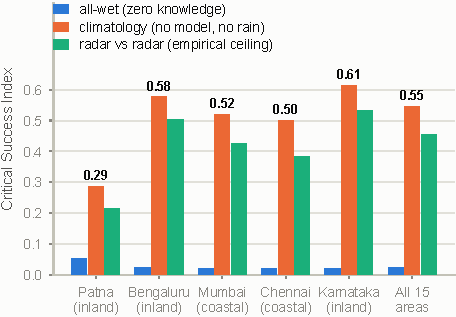
\includegraphics[width=\linewidth]{figures/f_csi_worth.pdf}
\caption{Table~\ref{tab:trivial} as a chart. In each of the five regions, climatology with one
fixed threshold and no physics or rainfall (orange) scores higher than the agreement between two
radar passes of the same city (green). Both are far above the all-wet baseline (blue) that this
literature usually compares against.}
\label{fig:worth}
\end{figure}

Table~\ref{tab:trivial} and Fig.~\ref{fig:worth} show the results. Climatology scores 0.29 to 0.67
per area, with a mean of 0.545. We do not know of any physics-based urban flood model scored against
Sentinel-1 that reports a higher CSI, and our own physics model scores far lower. In each of the
fifteen areas, climatology also scores higher than the agreement between two radar passes. This
makes sense once we think about it, because an average over many passes is more stable than any one
pass. It is a property of the radar data, and it limits what any model can be expected to achieve
here.

The score is this high because most of the water in these radar images has nothing to do with the
storm. Tidal flats, mangroves, seasonal ponds and paddy fields all appear as water, and the
permanent-water mask does not remove them. On this task, then, CSI mostly measures whether a method
can find standing water. Our physics model never tried to do that, because it predicts only the
water that the storm adds. The single-storm results support this reading. Mumbai-Northeast has one
real flood in our data, with 2\,937 wet cells compared with a usual level near 450. On that date
climatology scores 0.075, its worst value in the area. It does well on the quiet dates and badly on
the one flood. We therefore think that CSI on this task should always be reported next to all-wet
and a leave-one-out climatology computed on the same scenes. Without them the number is very hard to
interpret, and this includes the CSI of 0.041 that we published earlier.

\section{The Physics Model and a Learned Model}
\label{sec:twin}
We now compare methods on 18 monsoon storms in Patna and Mumbai-Northeast. All methods use the same
60\,m grid, the same mask and the same radar target, and permanent water is masked out of both the
prediction and the target. The storms are split into folds. In each fold some storms are held out
for testing and the rest are used for training, and every threshold is chosen on the training
storms of the fold, never on the scene being scored.

\begin{table}[!t]
\centering
\caption{All methods on the same 18 storms. No threshold is chosen on the scene being scored. The
learned model is a U-Net with 7.9\,M parameters that reads 23 terrain channels, with rainfall
removed, and its score is averaged over 3 seeds.}
\label{tab:baselines}
\begin{tabular}{lcc}
\toprule
method & mean CSI & $\times$ all-wet \\
\midrule
random                          & 0.014 & 0.5 \\
all-wet                         & 0.029 & 1.0 \\
best static index (HAND, TWI)   & 0.039 & 1.3 \\
physics twin (antecedent rain)  & 0.054 & 1.9 \\
\midrule
\textbf{learned (terrain only)} & \textbf{0.288 $\pm$ 0.007} & \textbf{9.9} \\
climatology (no model, no rain) & 0.288 & 9.9 \\
\bottomrule
\end{tabular}
\end{table}

\begin{figure}[!t]
\centering
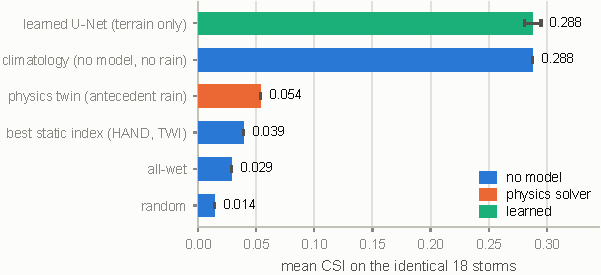
\includegraphics[width=\linewidth]{figures/f_method_ladder.pdf}
\caption{Table~\ref{tab:baselines} as a chart. A U-Net that reads the same terrain maps (green)
scores 5.4 times higher than the physics solver (orange). Climatology, which learns nothing, reaches
the same score as the U-Net.}
\label{fig:ladder}
\end{figure}

Table~\ref{tab:baselines} lists the results. Random scores 0.014 and all-wet scores 0.029. Static
terrain indices rank cells by the shape of the ground alone. The best of them scores 0.039. These are
HAND, the height of a cell above the nearest drainage line, and TWI, the topographic wetness index,
which grows with the area draining into a cell and falls with its slope. Our physics model, run with
the rain that fell in the days before each radar pass, scores 0.054. We then trained a U-Net to
read the same elevation, land cover and soil maps directly, with rainfall removed. It scores $0.288
\pm 0.007$ over three random seeds, which is 5.4 times the physics model on identical scenes. We had
earlier claimed that these terrain maps do not contain enough information to place a flood. This
result shows that the claim was wrong. The information is in the maps, and what fails is routing
water over a noisy elevation map with a solver.

The input that helps the most is available to both methods. It is the elevation minus a blurred copy
of itself, taken at blur widths of 2, 8 and 32 cells. FABDEM's errors are spatially correlated,
meaning that neighbouring cells tend to be wrong by similar amounts. Subtracting a blurred copy
cancels most of this shared error and keeps the small local rises and dips that decide where water
collects.

However, the learned model scores 0.2884 and climatology scores 0.2881. The difference is 0.0003,
while the standard deviation across training runs with different random seeds is 0.0066. On a city
that already has a radar archive, the network adds nothing over the plain statement that these
cells are usually wet. Its advantage is that it can run on a city with no radar archive, where
climatology cannot be computed. Section~\ref{sec:transfer} tests this.

\begin{figure}[!t]
\centering

\includegraphics[width=\linewidth]{figures/flood_uncertainty.png}
\caption{Ten simulations of Patna at 100\,mm, each on an elevation map with noise drawn from
FABDEM's own error class. Left, the fraction of runs in which each cell floods, from white (almost
none) to dark blue (almost all). Right, the spread in predicted depth. The total flooded area is
stable at $10.79 \pm 0.35$\,km$^2$, but only 5\,\% of Patna's flooded area floods in nine runs out of
ten. The size of the flood is well determined and its position is not.}
\label{fig:uncertainty}
\end{figure}

\subsection{Why the Physics Model Fails}
We ran the physics model on ten versions of the Patna elevation map. Each version adds spatially
correlated noise that matches FABDEM's stated error of about 1\,m \cite{marsh2024}. For a 100\,mm
storm, the total flooded area is stable at $10.79 \pm 0.35$\,km$^2$ (Fig.~\ref{fig:uncertainty}).
However, only 5\,\% of that area floods in at least nine of the ten runs. In Bengaluru, where the
ground has ten times more relief, the figure is 52\,\%. We also tuned 16 roughness and infiltration
multipliers, one for each land cover class, by gradient descent through the solver. This moved the
held-out CSI only from 0.0483 to 0.0488. These parameters change how deep the water gets, and they
have little effect on where it goes. When the elevation error is larger than the height differences
that decide which street floods, a solver that moves water downhill cannot put it in the right
place.

\begin{figure*}[!t]
\centering
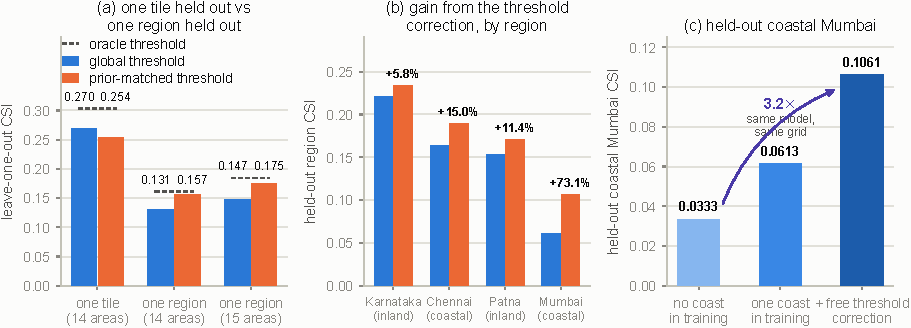
\includegraphics[width=\textwidth]{figures/f_transfer.pdf}
\caption{Results of Section~\ref{sec:transfer}. (a) The same model scores 0.270 or 0.147 depending
only on whether other areas from the same region remain in training. Dashed lines mark an oracle
threshold chosen by looking at the answer, and the prior-matched threshold (orange) closes most of
the gap to it. (b) The gain from this threshold correction for each held-out region. It is largest,
at $+73\,\%$, for Mumbai, where the model is weakest. (c) Held-out coastal Mumbai with no coastal
city in training, with one, and with the threshold correction added.}
\label{fig:transfer}
\end{figure*}

\section{Transfer to New Places}
\label{sec:transfer}
Climatology needs a radar archive of the city it describes. A city with no Sentinel-1 history has
no such archive, so the useful question is how well the learned model does on ground it has never
seen.

\subsection{Holding Out a Tile or a Region}
When we hold out one tile at a time, the model scores $0.270 \pm 0.015$, which is 12.5 times
all-wet. This number is misleading. The dataset has six Mumbai tiles and seven Karnataka areas.
Holding out Mumbai-West leaves the five neighbouring Mumbai tiles in training, and holding out
Chitradurga leaves six other Karnataka areas with the same climate and similar tanks. This tests new
ground inside a region the model already knows. When we hold out a whole region instead, the score
is $0.147 \pm 0.008$ (Fig.~\ref{fig:transfer}a). That is about half the per-tile figure and 6.9
times all-wet, and it is the number we expect in deployment. We also rebuilt the dataset between our
earlier three-area result of $0.094 \pm 0.021$ and this one. To check that the rebuild did not
cause the gain, we re-ran the same three areas on the new dataset and got $0.096 \pm 0.009$. The
gain therefore comes from having more areas.

Transfer is uneven across regions. Held out as whole regions, the seven Karnataka areas score 0.213,
which is 10.3 times all-wet, and Patna scores 0.166. The six Mumbai tiles score only 0.033, which is
close to predicting nothing. Most of the radar water in Mumbai is tidal flat, creek and mangrove, and
neither the Ganges flood plain nor the Karnataka plateau has any ground like it. This left two
possible explanations. Either coastal ground needs coastal training data, or tidal water cannot be
predicted from terrain at all.

\subsection{Adding a Coastal City}
To separate the two, we built a fifteenth area, Chennai. Chennai is 1\,300\,km from Mumbai and
shares no catchment with it. We kept it as a separate region, so that Chennai's fold trains with
Mumbai in the data and Mumbai's fold trains with Chennai. One experiment then tests both directions.

Building this area exposed a bug. Our scene selector had the monsoon hard-coded as 1 June to 15
October. India has two monsoons, and Chennai floods in the northeast monsoon from October to
December, so every scene we could request for Chennai came from its dry season. After the fix, the
wettest available date went from 40.3 to 180.5\,mm of rain in the days before the pass. One date
turned out to have five to ten times the wet fraction of any other Chennai scene. It was a real
flood that the old selection could not reach. The season window is part of the experiment design,
and it should be checked for every city.

With Chennai in training, held-out Mumbai rises from 0.033 to 0.061. Chennai, with Mumbai in
training, scores 0.164, which is 7.8 times all-wet. That is close to inland Karnataka's 10.6 times
and far above the 1.8 times that Mumbai reached as the only coastal city. Tidal water can therefore
be learned from terrain, as long as the model has seen a coast. The experiment carries its own
control. Every fold gained the same ten storms, but only the coastal region changed much, by
$+84\,\%$ on the coast against $+3.6\,\%$ for Karnataka and $-7.4\,\%$ for Patna. The overall score
rose from 0.131 to 0.147. These ten storms added 13\,\% more data and nearly doubled the score for
one region. In practice, the model can be used on a new inland city, but on a new coastal city only
when a coastal city is in the training data.

\subsection{A Threshold Correction}
The model gives each cell a probability of being wet, and a threshold turns these probabilities into
a wet or dry map. We measure ranking quality as the best CSI the model could reach if its threshold
were chosen on the test scene itself. It shows how well the model orders cells from most to least
likely to flood, separately from the choice of threshold. In every experiment, ranking quality is
higher than the CSI actually achieved, so part of the error comes from the threshold. A simple fix
is available. For each test scene, we choose the threshold so that the predicted wet fraction equals
the mean observed wet fraction of the training scenes. This uses no test labels. On the
leave-one-region-out split it raises CSI from 0.1474 to 0.1746 with 15 areas, and from 0.1305 to
0.1566 with 14. These gains are 3.4 and 5.7 seed standard deviations, and they close 73 and 84\,\%
of the gap to an oracle threshold chosen while looking at the test scene.

On the per-tile split the same correction lowers CSI, from 0.2698 to 0.2542. We think this change of
sign is real and has a simple cause. When one tile is held out, its sibling tiles are still in
training, so the training wet fraction already fits it. A whole held-out region has no such
siblings, and its default threshold is off. For the same reason the correction helps most where the
model is weakest, with $+73\,\%$ for coastal Mumbai against $+5.8\,\%$ for Karnataka
(Fig.~\ref{fig:transfer}b). At the default threshold the model finds only half to four-fifths of the
water that is really there, and for a flood product, missing water is the worse error. Taken
together, held-out coastal Mumbai went from 0.033 with no coast in training, to 0.061 with one
coastal city, to 0.106 with the correction (Fig.~\ref{fig:transfer}c). This is 3.2 times the
starting score, reached with the same model size and the same grid.

\begin{figure*}[!t]
\centering
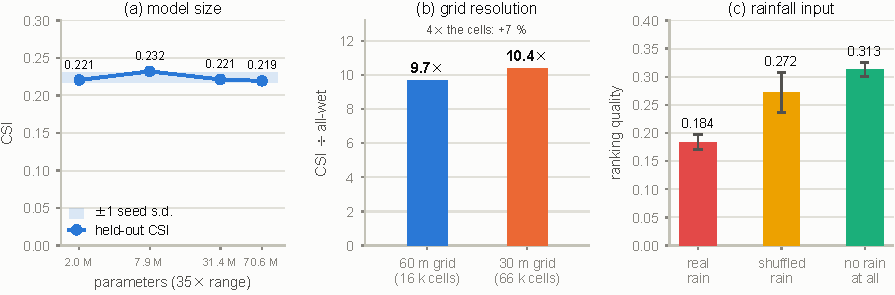
\includegraphics[width=\textwidth]{figures/f_nonlevers.pdf}
\caption{Three changes that did not help. All axes start at zero so that small differences are not
exaggerated. (a) A 35-fold range in model size. The shaded band is one seed standard deviation around
the mean. (b) Four times as many cells raises the score, measured as a multiple of
all-wet, by 7\,\%. We use this multiple because raw CSI is not comparable across grids. (c) Ranking
quality with real rainfall, with rainfall shuffled between storms, and with no rainfall. Real
rainfall gives the worst result.}
\label{fig:nonlevers}
\end{figure*}

\section{Changes That Did Not Help}
\label{sec:levers}
When a model does poorly, the usual response is to make it bigger, give it a finer grid, or give it
more inputs. We tried all three and none of them helped (Fig.~\ref{fig:nonlevers}). We report them
because they are the first things others are likely to try.

\subsection{Model Size}
On held-out floods with terrain inputs only, CSI is 0.221 at 2.0\,M parameters, 0.232 at 7.9\,M,
0.221 at 31.4\,M and 0.219 at 70.6\,M. Over a 35-fold range in size, the differences stay within
seed noise.

\subsection{Grid Resolution}
Running at 30\,m instead of 60\,m gives four times as many cells. The score is 10.4 times all-wet at
30\,m, against 9.7 times at 60\,m. We compare multiples of all-wet here because raw CSI values from
different grids are not directly comparable.

\subsection{Rainfall}
Removing the rainfall inputs improves ranking quality by 0.129. That is about seven seed standard
deviations, and the ranges over three seeds do not overlap. We also shuffled the rainfall between
storms, which keeps every rainfall value but breaks the link between each storm and its own rain.
Ranking quality is 0.184 with real rain, 0.272 with shuffled rain and 0.313 with no rain, so real
rainfall gives the worst result of the three. We tested and ruled out two other explanations, tidal
differences between the Mumbai tiles and a failure to extrapolate to larger storms. On an unseen
region rainfall makes almost no difference, with a CSI of 0.1460 with rain and 0.1474 without. So
rainfall does not always hurt. On a city the model has already seen, it gives the model a shortcut,
and that shortcut does not carry over to new ground. The free rainfall data also has almost no
spatial detail at this scale. Nine probe points spread across a 15\,km tile all fall into the same
cell of the rainfall archive, so the model gets a single rainfall series for the whole tile.

\section{Planning}
\label{sec:planning}
Section~\ref{sec:twin} showed that the model cannot reliably say which street floods first.
Planning still works, because a plan depends mainly on how much water there is and where it can
drain, and the model is stable on these. Across the ten noisy elevation maps, for example, the total
flooded area varied by only about 3\,\%. Every intervention is tested in the same way. We change the
terrain, run the 100\,mm design storm again for 24 hours, and measure flooding on built-up cells. The
intervention's own cells are removed from both the before and the after masks, so moving water into
a drain is not counted as removing it.

\begin{figure}[!t]
\centering
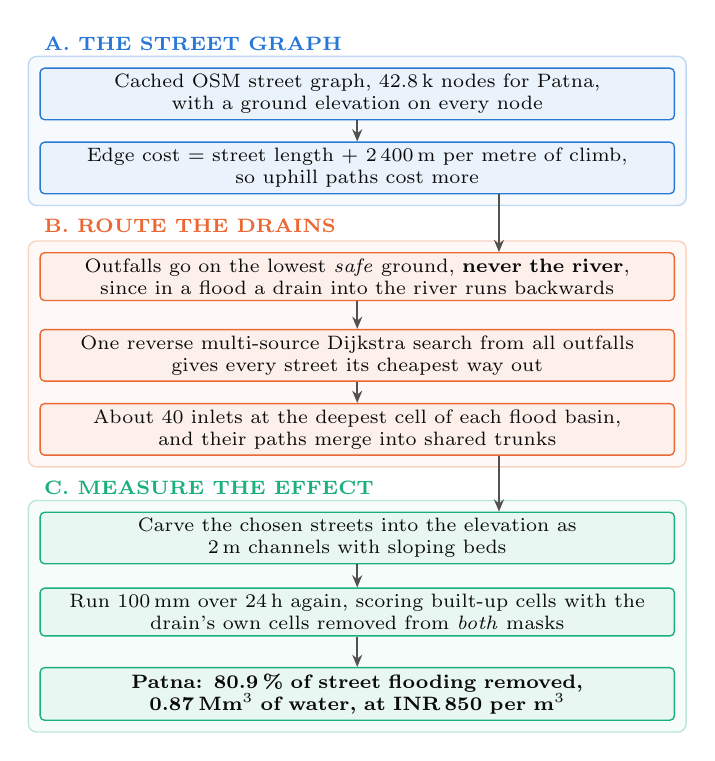
\begin{tikzpicture}[x=1cm,y=1cm]

\node[vhead=vblue,anchor=west] at (-0.2,0.34) {A. THE STREET GRAPH};
\node[vbox=vblue,text width=7.9cm] (g1) at (3.9,-0.30)
  {Cached OSM street graph, 42.8\,k nodes for Patna,\\with a ground elevation on every node};
\node[vbox=vblue,text width=7.9cm] (g2) at (3.9,-1.24)
  {Edge cost $=$ street length $+$ 2\,400\,m per metre of climb,\\so uphill paths cost more};

\node[vhead=vorange,anchor=west] at (-0.2,-1.98) {B. ROUTE THE DRAINS};
\node[vbox=vorange,text width=7.9cm] (r1) at (3.9,-2.62)
  {Outfalls go on the lowest \emph{safe} ground, \textbf{never the river},\\since in a flood a drain into the river runs backwards};
\node[vbox=vorange,text width=7.9cm] (r2) at (3.9,-3.62)
  {One reverse multi-source Dijkstra search from all outfalls\\gives every street its cheapest way out};
\node[vbox=vorange,text width=7.9cm] (r3) at (3.9,-4.56)
  {About 40 inlets at the deepest cell of each flood basin,\\and their paths merge into shared trunks};

\node[vhead=vaqua,anchor=west] at (-0.2,-5.30) {C. MEASURE THE EFFECT};
\node[vbox=vaqua,text width=7.9cm] (v1) at (3.9,-5.94)
  {Carve the chosen streets into the elevation as\\2\,m channels with sloping beds};
\node[vbox=vaqua,text width=7.9cm] (v2) at (3.9,-6.88)
  {Run 100\,mm over 24\,h again, scoring built-up cells with the\\drain's own cells removed from \emph{both} masks};
\node[vbox=vaqua,text width=7.9cm] (v3) at (3.9,-7.92)
  {\textbf{Patna: 80.9\,\% of street flooding removed,}\\\textbf{0.87\,Mm$^3$ of water, at \rupee850 per m$^3$}};

\begin{pgfonlayer}{background}
  \node[vband=vblue,  fit=(g1)(g2)] {};
  \node[vband=vorange,fit=(r1)(r3)] {};
  \node[vband=vaqua,  fit=(v1)(v3)] {};
\end{pgfonlayer}

\foreach \a/\b in {g1/g2, r1/r2, r2/r3, v1/v2, v2/v3}
  \draw[vflow] (\a.south) -- (\b.north);
\draw[vflow] ($(g2.south)+(1.8,0)$) -- ($(r1.north)+(1.8,0)$);
\draw[vflow] ($(r3.south)+(1.8,0)$) -- ($(v1.north)+(1.8,0)$);

\end{tikzpicture}
\caption{How the drain network is designed and scored. (A) The street graph and its edge costs. (B)
One graph search from all outfalls gives every street its cheapest exit, and the paths from about 40
inlets form the network. (C) The network is carved into the terrain and the storm is run again. The
drain's own cells are removed from both the before and the after mask, so the planner gets no credit
for moving water into the drain.}
\label{fig:spideralg}
\end{figure}

\subsection{Storm Drain Network}
Our earlier planner built sparse canals, each running from the worst flood basin to the nearest
outfall. A lot of real drainage retrofitting follows the same pattern. These canals cut street
flooding by 20.8\,\% in Patna and 25.7\,\% in Bengaluru. The new planner builds a dense network
along the real streets (Fig.~\ref{fig:spideralg}). The street graph for Patna has 42.8\,k nodes,
each with a ground elevation. The cost of a street segment is its length plus 2\,400\,m for every
metre it climbs, so uphill paths are expensive. We run one reverse multi-source Dijkstra search from
all outfalls at once. Dijkstra's algorithm finds the cheapest path through a graph, and running it
backwards from every outfall together gives each street its cheapest way out. We then place about 40
inlets at the deepest cell of each flood basin and follow each inlet's path to its outfall. The
paths merge into shared trunk drains that carry the flow of several basins. Outfalls are never
placed on the river, because in a flood the river runs high and a drain into it would flow
backwards. The search uses the lowest safe ground instead. Finally, the chosen streets are carved
into the elevation as 2\,m channels with sloping beds, and the storm is run again.
Fig.~\ref{fig:spidermap} shows the resulting network in Patna.

\begin{figure}[!t]
\centering
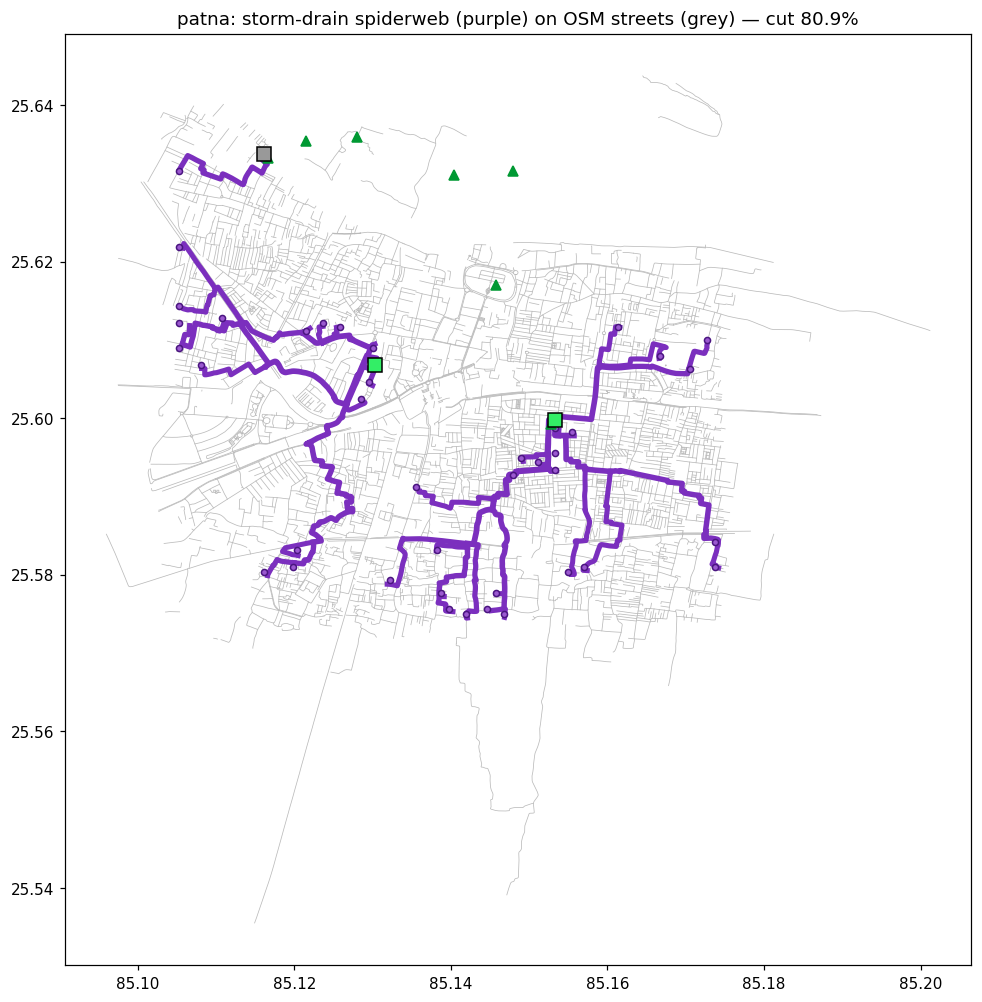
\includegraphics[width=0.82\linewidth]{figures/spiderweb_patna.png}
\caption{The drain network of Fig.~\ref{fig:spideralg} in Patna. Grey is the OpenStreetMap street
network. Purple is the chosen drain, drawn thicker where more basins share a trunk, and the small
purple dots are inlets. Green squares are the lowland outfalls chosen by the search, and green
triangles are river outfalls it was not allowed to use. The whole network comes from the search,
with no manual drawing.}
\label{fig:spidermap}
\end{figure}

Across the eight areas where we built it, the network cuts street flooding by 80.9\,\% in Patna,
89.4\,\% in Patna-East, 80.3\,\% in Patna-West and 72.6\,\% in Bengaluru. On the four largest Mumbai
tiles it cuts 32.5 to 63.0\,\%. The sparse plans cut 21 to 26\,\%. We also ran storms from 25 to
200\,mm, and the response rises steadily with storm depth. For Patna, the dense network removes 0.87
million m$^3$ of flood water, against 0.28 million for the sparse plan. It is also cheaper per unit
of water removed, at \rupee850 per cubic metre against \rupee1\,309, because each shared trunk serves
many basins. For comparison, excavation at eight sites cuts flooding by 4.1\,\%, detention pits by
7.8\,\%, and 727 distributed storage basins by 30\,\% at \rupee9\,200 per cubic metre
(Fig.~\ref{fig:planning}). The Mumbai tiles gain less because they are four times larger and partly
harbour, so a fixed budget of 40 inlets covers a smaller share of their flooding.

\begin{figure*}[!t]
\centering
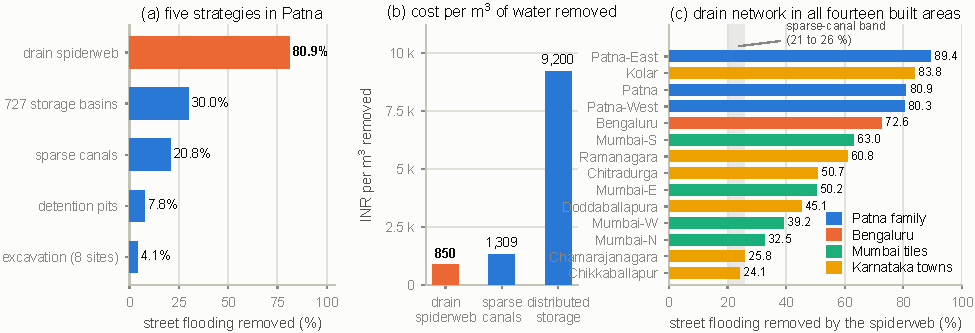
\includegraphics[width=\textwidth]{figures/f_planning.pdf}
\caption{Planning results, all measured by running the storm again. (a) Five strategies in Patna.
The dense drain network removes about four times as much street flooding as sparse canals. (b) Cost
per cubic metre of water removed. The dense network is also the cheapest, because its shared trunks
serve many basins. (c) The same planner, unchanged, on all fourteen built areas. The grey band marks
what the sparse plans achieve, and only two areas fall inside it.}
\label{fig:planning}
\end{figure*}

\subsection{Storage and Recharge}
A separate storage planner ranks sites for detention tanks by how deep water pools at local low
points. It skips building footprints, since a tank cannot be dug under a house. The planner has
never seen a flood report or a news article, but its top sites fall on each city's well-known flood
spots. These include Koramangala in Bengaluru, and the Parel and Byculla area in Mumbai, where the
municipal corporation has built underground tanks.

The water that floods an Indian city in July is water the same region is short of in April. Most
recharge plans assume an infiltration rate and multiply it by an area. Our model already tracks
infiltration against a finite soil capacity, so we can build recharge structures into the terrain,
run the storm, and read off how much water actually went underground. We first choose where to
build. We screen all 27 district units of Karnataka with four free datasets. The Central Ground
Water Board reports the stage of extraction, which is the share of each year's recharge that is
pumped out. We add a groundwater storage trend from the GRACE satellites, flow accumulation from
HydroSHEDS and soil conductivity from SoilGrids. Five districts rank highest, with extraction of 111
to 187\,\%, and all five are officially classed as over-exploited or critical.

Across the fourteen built areas, the results fall into two clear groups (Fig.~\ref{fig:recharge}).
The six Karnataka towns send 6.3 to 16.5\,\% of a 100\,mm storm's runoff into the aquifer.
Chikkaballapur and Kolar lead, with 607\,172 and 667\,548\,m$^3$. The other eight
areas, on the Patna flood plain, in Bengaluru and on the Mumbai coast, send 3.3\,\% or less, and
Mumbai-South sends almost none. This split is what the screen predicted, and it has a physical
cause. On a flood plain the water table is already near the surface and the soil is nearly full, so
there is no room for more water. On the Karnataka plateau the aquifer has been pumped down and hard
rock lies under thin soil, so there is empty storage to fill. In these towns the same structures
also remove 46.9 to 88.2\,\% of street flooding. Where recharge works, it helps with floods and with
water supply at the same time.

\begin{figure*}[!t]
\centering
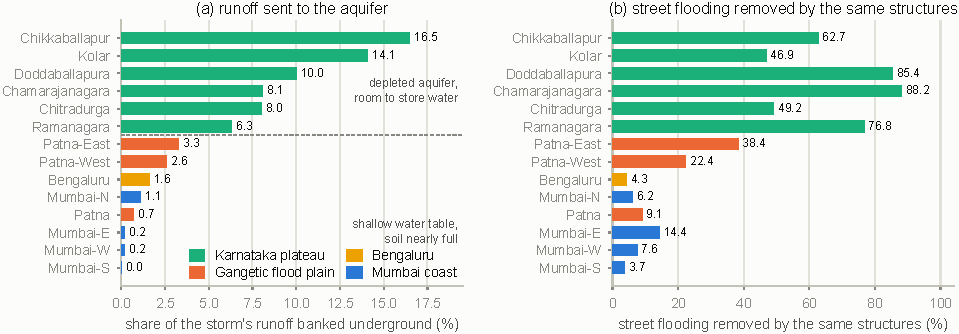
\includegraphics[width=\textwidth]{figures/f_recharge.pdf}
\caption{Recharge measured by simulation in all fourteen built areas. (a) The share of a 100\,mm
storm's runoff that reaches the aquifer after the structures are built. The six Karnataka plateau
towns, above the dashed line, send 6.3 to 16.5\,\% underground because their aquifer is depleted and
the soil has room. The other areas send 3.3\,\% or less because their soil is already close to
full. (b) The same structures remove 46.9 to 88.2\,\% of street flooding in the Karnataka towns.}
\label{fig:recharge}
\end{figure*}

\subsection{Drainage Inferred From Radar}
The largest known gap in the twin is that it has no storm sewers, so it floods too much wherever
working drains exist. Mumbai's drainage map is not public. Instead, we fit an outflow map, with one
value per cell for how much water that cell drains away, by gradient descent through the simulator
on 8 storms, and we test it on 3 others. A penalty on every cubic metre drained makes the fit choose
the smallest drainage that explains the observed flood extent, so every volume it gives is a lower
bound. On the held-out storms the extent score improves by 10\,\% while the number of predicted wet
cells falls by 10\,\%. A higher CSI usually comes from predicting more water, so this is the more
convincing direction. Adding up the drained volume gives Mumbai's total surface outflow as at least
3.48 million m$^3$ for a 25\,mm storm, rising only to 5.41 million m$^3$ at 200\,mm. Outflow levels
off while the flooded area keeps growing, which predicts a ceiling of about 5.4 million m$^3$ per
storm that can be checked against records. The municipal corporation reported pumping about 4.7
million m$^3$ per day through six pumping stations from 16 to 19 August 2025. Our lower bound for
total outflow sits just above this pumped figure. That is the expected side, since our outflow also
includes drains that work by gravity. This is a consistency check and not a validation.

\begin{figure}[!t]
\centering
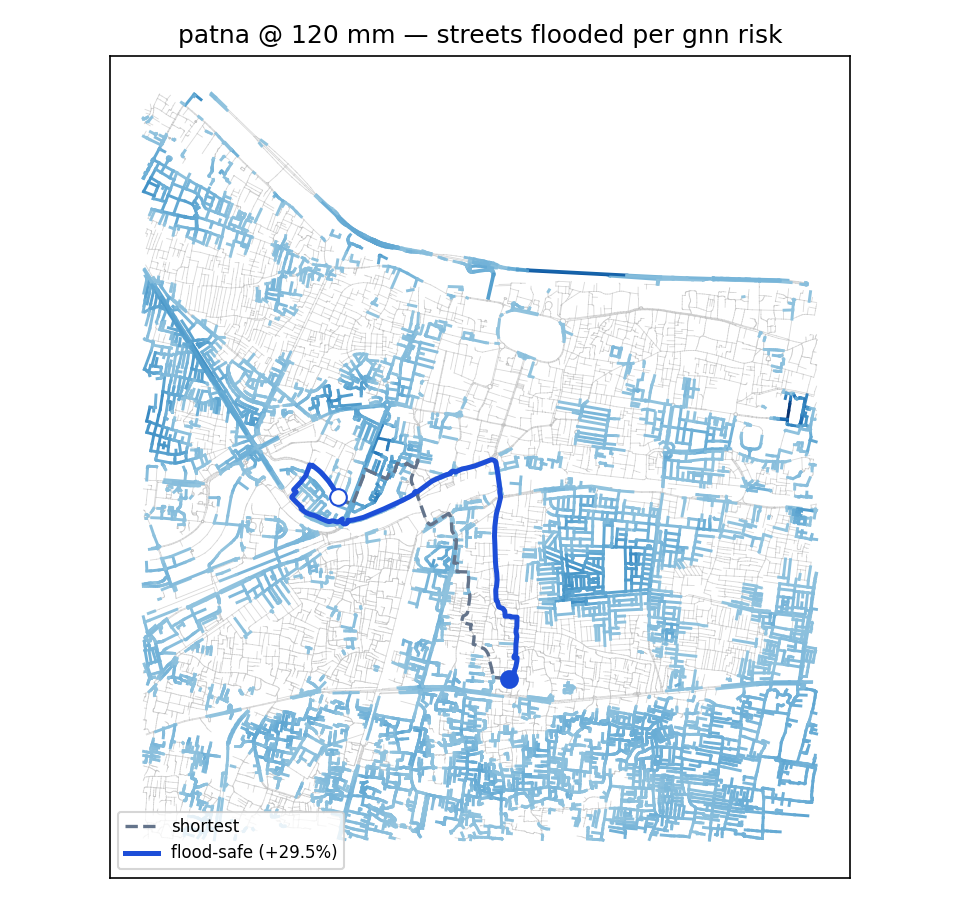
\includegraphics[width=0.80\linewidth]{figures/route_demo_patna.png}
\caption{Street-level risk in Patna under a 120\,mm storm. Each street is shaded by the risk that the
graph network gives it, with darker meaning more dangerous. The grey dashed line is the shortest walk
between two points, and the solid blue line avoids floodwater at the cost of 29.5\,\% more distance.
Computing the risk takes about 4\,ms, against 260\,ms for the raster pipeline it was trained to
copy.}
\label{fig:route}
\end{figure}

\subsection{Street-Level Risk and Routing}
A planner asks where to build. A person out in the rain asks which way to walk. For this we trained a
message-passing network on the street graph. This is a graph neural network in which each street
node repeatedly updates its state from its neighbours. Given the rainfall, it learns to reproduce
the twin's flood risk for each street. On held-out storm sizes it reaches an AUC of 0.890 to 0.942,
where AUC is the probability that a randomly chosen flooded street is ranked above a randomly chosen
dry one. It takes about 4\,ms, against 260\,ms for the raster pipeline it was trained to copy. With
Bengaluru left out of training entirely, it still ranks that city's flooded streets at an AUC of
0.721, so performance drops on an unseen city, as it did for the radar model in
Section~\ref{sec:transfer}. We then route trips on a street cost that is raised by flood risk.
Judged on the simulated depths over 150 random trips in Patna, these routes achieve 64.6\,\% of the
flood avoidance of an oracle router that knows the true depths, while adding 57\,\% of the oracle's
extra distance. Fig.~\ref{fig:route} shows one such route.

\section{Limitations}
\label{sec:limits}
The hydraulics run on 60\,m cells, which are coarser than the streets they describe. We compared the
twin with 83 crowdsourced depth reports from the public mumbaiflood.in service, which were kept out
of all fitting. The twin under-predicts depth by a steady factor of 4.45. If each real pond is
spread over a whole 60\,m cell in the model, this factor suggests that real ponds are about 28.5\,m
across. A finer grid is the clearest next step, and this gives it a concrete target. At these report
locations the correlation between predicted and observed depth is near zero, which is the same
difficulty in placing water that we found with radar.

The evidence is also uneven. Table~\ref{tab:baselines} rests on 18 storms in two areas, while the
baseline and transfer results rest on 15 areas and 150 scenes. The Mumbai tiles are separate models
with closed boundaries, so flow across tile edges and tides are missing, and the coastal result
rests on only two cities. Recharge volumes come from the model's own infiltration accounting, but
the ranking of sites within a town uses placeholder groundwater data, and recharge also affects
water quality, which a flood model cannot see. Costs are rough. They are meant for ranking
strategies and not for pricing projects. The planner is a tool for setting priorities, and any
design it proposes still needs engineering checks.

\section{Conclusion}
\label{sec:conclusion}
Our main recommendation concerns how flood models are scored. On this task a flood overlap score
means little by itself. A baseline with no physics, no rainfall and one fixed parameter scores 0.29
to 0.67 across 15 areas. It beats every physics-model score we could find, and in all fifteen areas
it beats the agreement between two radar passes of the same city. Any CSI on this task, including
ours, should be read next to these numbers.

Read this way, our physics twin scores 0.054 and a learned model on the same maps scores 0.288. The
learned model ties the baseline on cities that have a radar archive, so its use is on cities that do
not. There it scores 0.147 with a whole region held out, and 0.175 with a threshold correction that
costs nothing. Its weakest case is a coast it has not seen, and adding one coastal city to training
fixes much of that. Planning holds up despite the uncertainty in where water collects, because every
intervention is measured by running the storm again. The clearest next steps are a finer grid and
more coastal cities in training.

\section*{Code, Data and Acknowledgment}
The code and every per-area bundle, including the Sentinel-1 water masks, road graphs and ranked
site lists, are public at \url{https://github.com/Maverick-Ansh/project-varuna}, together with
offline tests and run instructions. The live dashboard is at
\url{https://project-varuna-iota.vercel.app}. Every headline number can be regenerated from a
committed file. Rebuilding the whole dataset from scratch gives the same main result, $0.288 \pm
0.008$ against $0.288 \pm 0.007$. This work uses FABDEM, ESA WorldCover, JRC Global Surface Water,
Copernicus Sentinel-1, OpenStreetMap, Open-Meteo, SoilGrids, HydroSHEDS and Central Ground Water
Board data, all free to use, as well as crowdsourced observations from mumbaiflood.in. It runs on
the free tiers of Google Colab, Kaggle, Hugging Face and Vercel.

\balance
\bibliographystyle{IEEEtran}
\bibliography{varuna-ieee}

\end{document}
